\documentclass{article}

% Language setting
% Replace `english' with e.g. `spanish' to change the document language
\usepackage[english]{babel}

% Set page size and margins
% Replace `letterpaper' with`a4paper' for UK/EU standard size
\usepackage[letterpaper,top=2cm,bottom=2cm,left=3cm,right=3cm,marginparwidth=1.75cm]{geometry}

% Useful packages
\usepackage{amsmath}
\usepackage[colorlinks=true, allcolors=blue]{hyperref}

\usepackage{amsfonts}
\usepackage{amssymb,amsthm,amsmath}
\usepackage[shortlabels]{enumitem}
\usepackage{setspace}
\usepackage{tikz}
\usepackage{bbm}
\usepackage{multicol}
\usepackage{cancel}
\usepackage{graphicx}
\usepackage{booktabs}
\usepackage{extarrows}
\usepackage{mathrsfs}
\usepackage{algorithm}
\usepackage{algorithmic}


\title{ISMIR 2021 Paper Summary}
\author{Junchuan Zhao}

\begin{document}
\setstretch{1.2} 
\maketitle

\begin{abstract}
A summary of music generation papers accepted by ISMIR 2021. (Publicly Available)
\end{abstract}

\section{SURPRISENET: MELODY HARMONIZATION CONDITIONING ON USER-CONTROLLED SURPRISE CONTOURS}
SupriseNet Traits\\
(1) relieves trade-off between coherence, which caused by the melody and surprisingness, which caused by the user-supplied condition.\\
(2) the chords are correponded to the melody and follow the surprise contour.\\

\noindent
Transition matrix ($a \in \mathbb{R}^{N \times N}$): encode the distribution of the chord at this time given the previous element.\\
$p({\rm chord}_t|{\rm chord}_{t-1})$\\

\noindent
Surprisingness: equivalent to the definition of the information content in information theory.\\
${\rm Surprisingness} = -\log{p({\rm chord}_t|{\rm chord}_{t-1})}$.\\
The higher the surprise value at a certain time, the gerater the amount of information at that time.\\

\noindent
\begin{figure}[H]
	\centerline{
   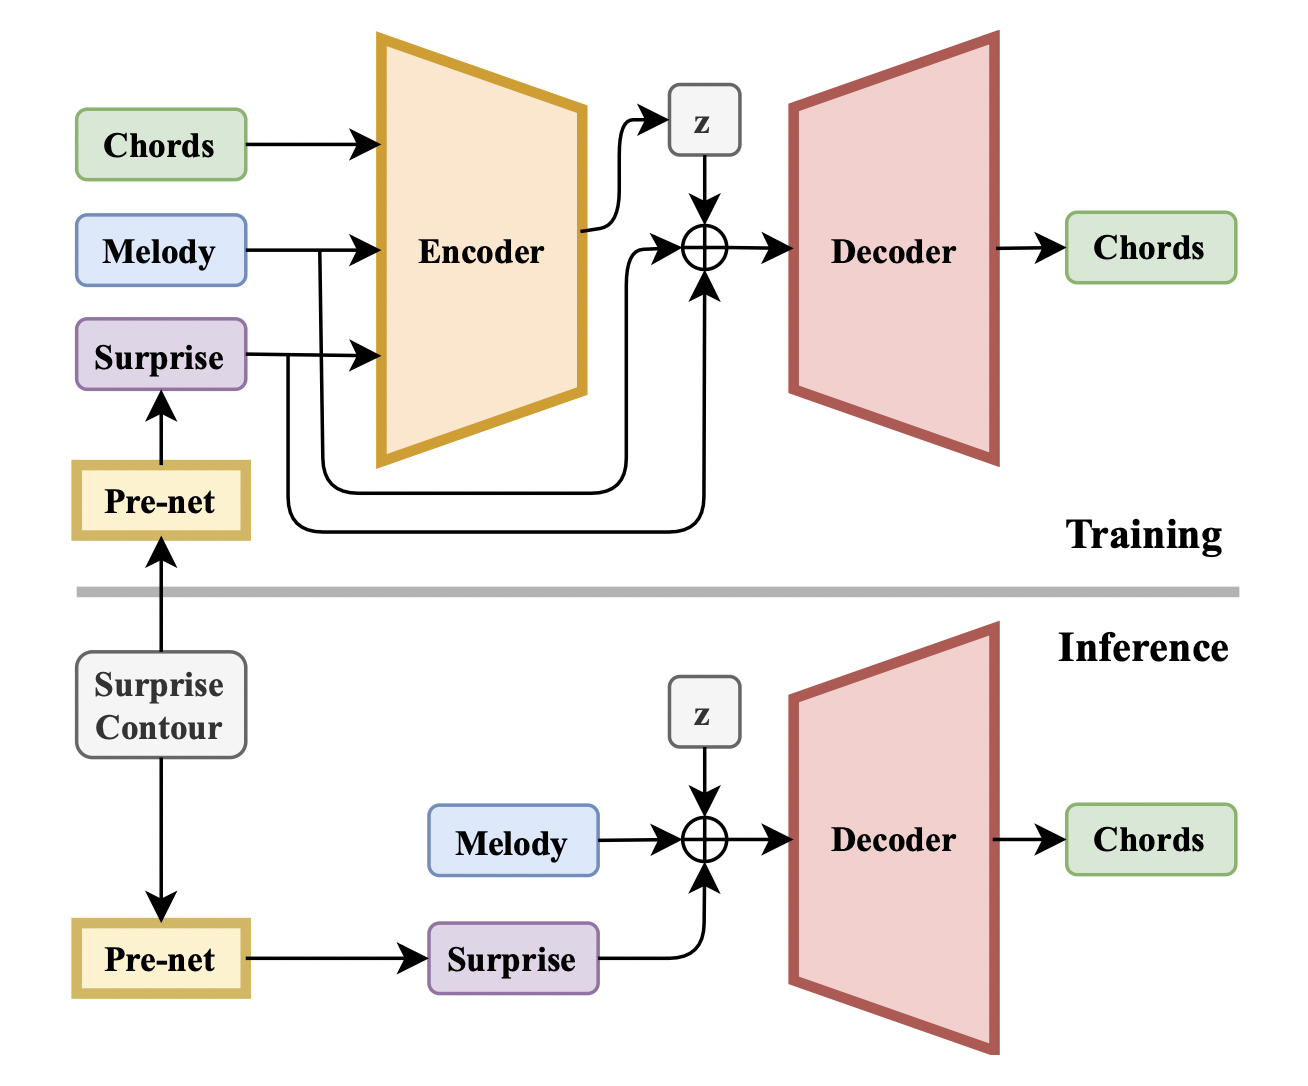
\includegraphics[width=0.5\textwidth]{Fig1.png}}
   \caption{The structure of SURPRISENET.}
   \label{fig:example}
\end{figure}

\noindent
\begin{figure}[H]
	\centerline{
   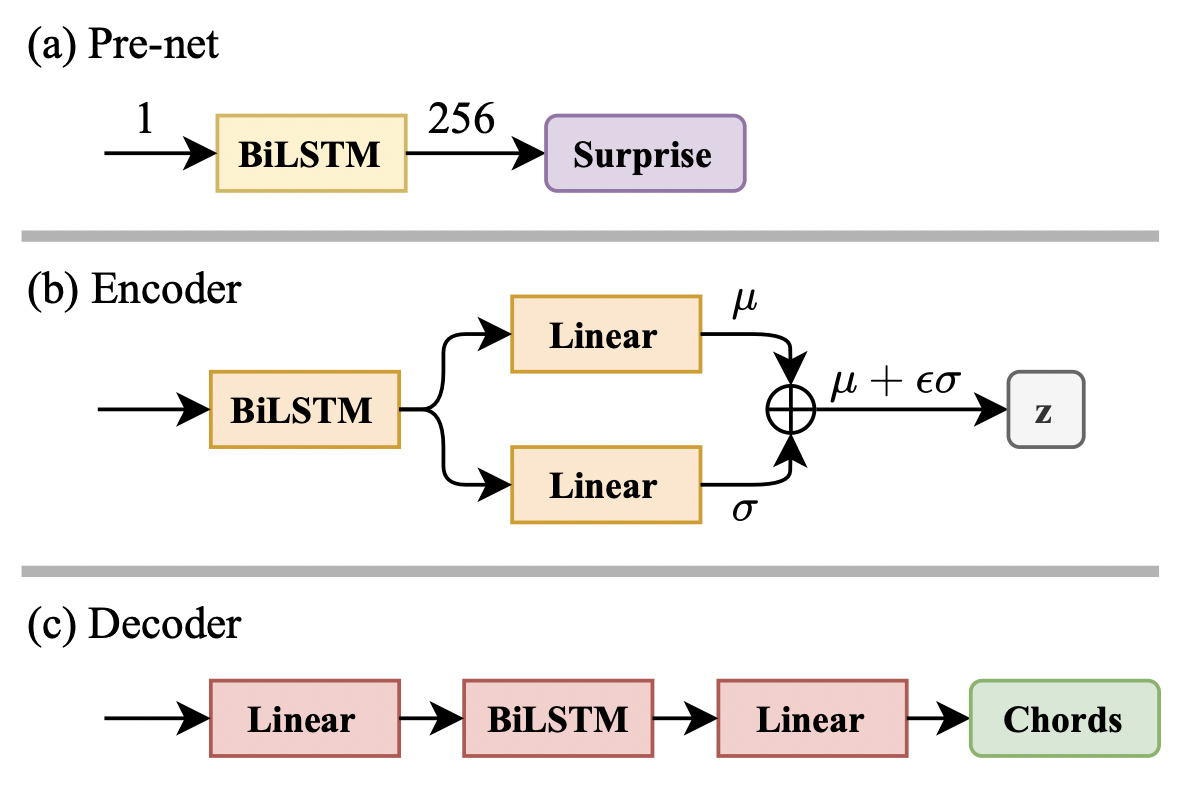
\includegraphics[width=0.5\textwidth]{Fig2.png}}
   \caption{Three main components of SURPRISENET.}
   \label{fig:example}
\end{figure}

\noindent
Pre-net: extend the feature from a scaler to a 256-dimensional vector.\\
CVAE: the features of the chord, melody, and extended surprise contour are concatenated and fed into the encoder to generate a latent code $z$ subject to standard normal distribution.\\

\noindent
Future work\\
(1) the meaning of surprise: chord, melody?\\
(2) the surprise contours, relationship between different surprise contours?\\
(3) sample the surprise contours that generate melodious music?\\
(4) surprisingness -- style classification.\\

\section{CONTROLLABLE DEEP MELODY GENERATION VIA HIERARCHICAL MUSIC STRUCTURE REPRESENTATION}
Problems\\
(1) model larger scale music structure and multiple levels of repetition\\
(2) controllability to create desired tempo, styles, and mood\\
(3) scarcity of training data\\

\noindent
1. MusicFrameworks\\
(1) high-level representation: repeated sections and phrases\\
(2) low-level representation: rhythm structure and melodic contour\\
2. Generate melodies from music frameworks\\
3. Achieve controllability by editing the music frameworks at any level
\begin{figure}[H]
	\centerline{
   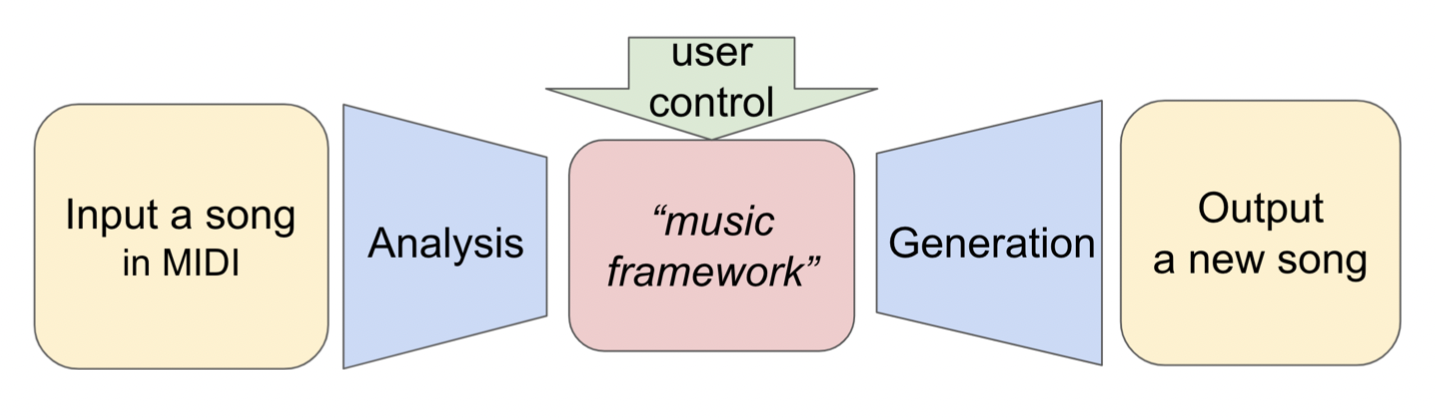
\includegraphics[width=0.5\textwidth]{Fig3.png}}
   \caption{Architecture of MusicFrameworks.}
   \label{fig:example}
\end{figure}

\noindent
Advantages of Music Frameworks
A new song can be generated using the structure from song A, basic melody from song B, and basic rhythm form from song C.\\

\noindent
Music Frameworks Analysis
\begin{figure}[H]
	\centerline{
   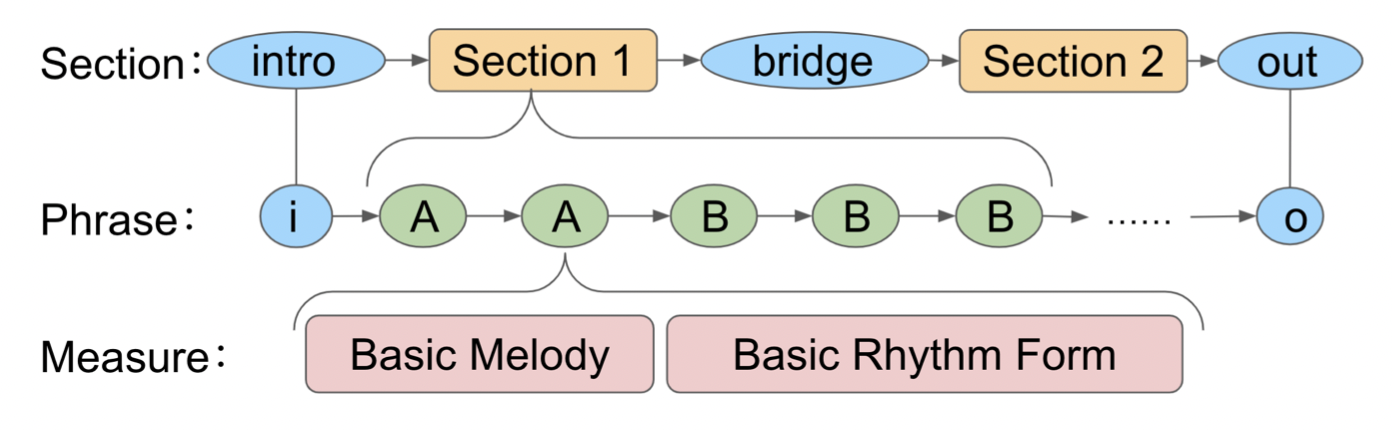
\includegraphics[width=0.5\textwidth]{Fig4.png}}
   \caption{An example music framework.}
   \label{fig:example}
\end{figure}
\noindent
(1) section and phrase-level structure analysis results\\
(2) basic melody and basic rhythm form within each phrase\\
\indent
Basic Melody: a sequence of half notes representing the most common pitch in each 2-beat segment of the original phrase\\
\indent
Basic rhythm form: consists of a per-measure descriptor with two components (a. pattern label; b. rhythmic complexity)\\

\noindent
Generation Using Music Frameworks\\
1. user or the library provides the section and phrase structure.\\
2. generate a basic melody, generate rhythm using the basic rhythm form.\\
3. generate a new melody given the basic melody.\\
\begin{figure}[H]
	\centerline{
   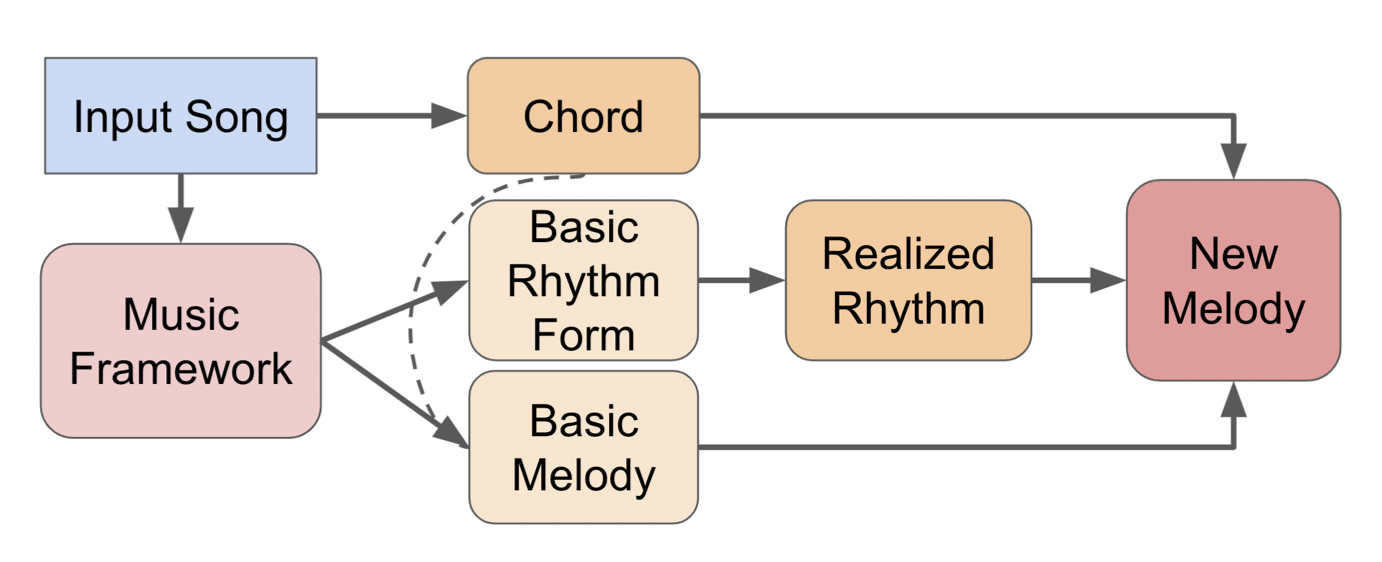
\includegraphics[width=0.5\textwidth]{Fig5.png}}
   \caption{Generation process from music frameworks within each phrase.}
   \label{fig:example}
\end{figure}

\noindent
Basic Melody Generation\\
input: $x_i = ({\rm pos}_i, c_i, ...)$\\
sampling with Dynamic Time Warping: melody contour rating function to estimate the contour similarity between two basic melodies.\\

\noindent
Realized Rhythm Generation\\
rhythm pattern: $r_i$ (256 possible rhythm patterns with a 2-beat length)\\
input: $x_i = (r_{i-1},{\rm brf}_i,{\rm pos}_i)$\\
beam search\\

\noindent
Realized Melody Generation\\
input: $x_i$ includes the current note's duration, the basic melody pitch, the current chord ($c_i$), three positional features (${\rm pos}_i$).\\

\noindent
Network Architecture
\begin{figure}[H]
	\centerline{
   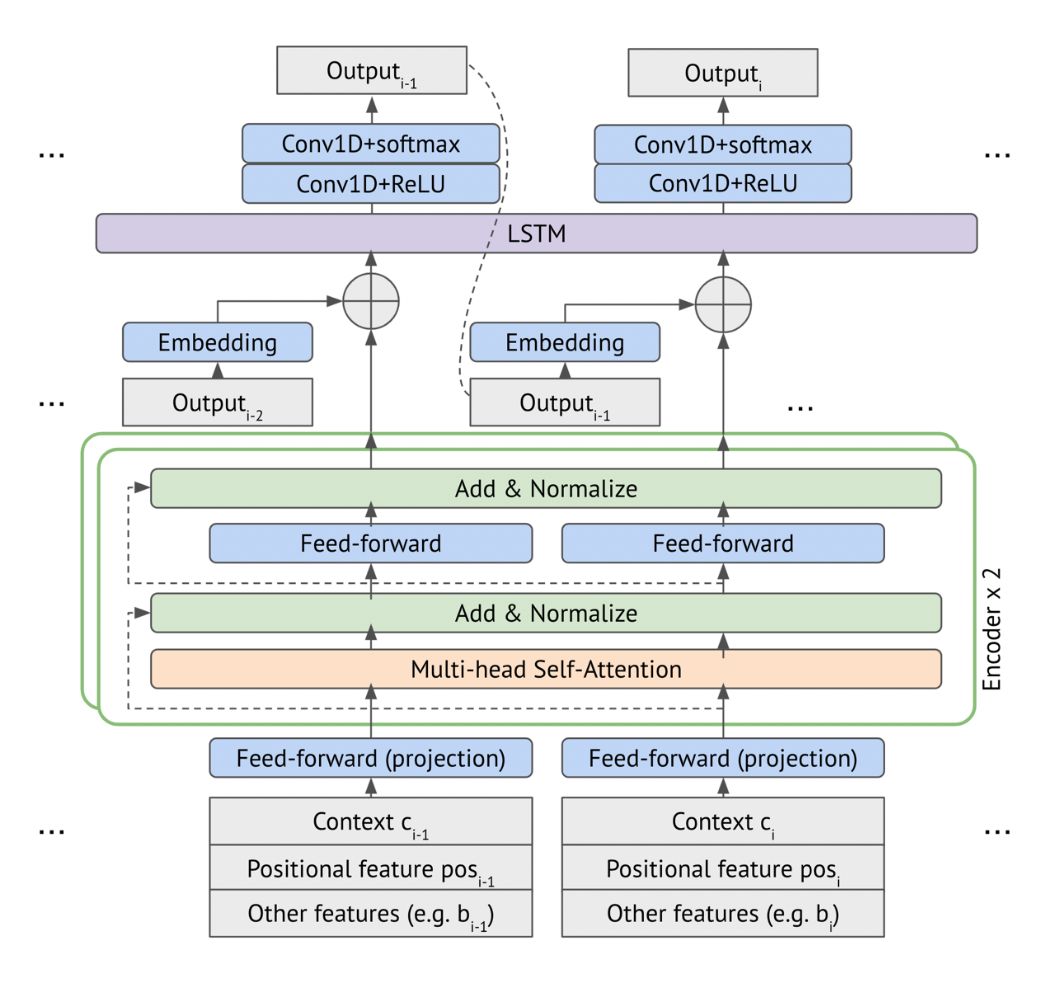
\includegraphics[width=0.5\textwidth]{Fig6.png}}
   \caption{Transformer-LSTM architecture for melody, basic melody and rhythmic pattern generation.}
   \label{fig:example}
\end{figure}

\noindent
Conclusion\\
(1) The key idea: adopt an abstract representation -- music frameworks (long term repetitive structures; phrase-level basic melodies and basic rhythm forms)\\
(2) Controllability: manipulation of music frameworks, can be edited and combined to guide compositions.\\

\section{MINGUS: MELODIC IMPROVISATION NEURAL GENERATOR USING SEQ2SEQ}
MINGUS relies on two dedicated embedding models (pitch and duration) and exploits in prediction features such as chords (current and following), bass line, position inside the measure.\\

\noindent
Data representation\\
P: ${\rm [0-128]}$, D: ${\rm [0-12]}$, C (Chord): ${\rm [0-128\times4]}$, NC (Next Chord): ${\rm [0-128\times4]}$, B: {\rm [0-128]},  BE: {\rm [0-3]}, O: {\rm [0-95]}\\

\noindent
Model Architecture
\begin{figure}[H]
   \centerline{
   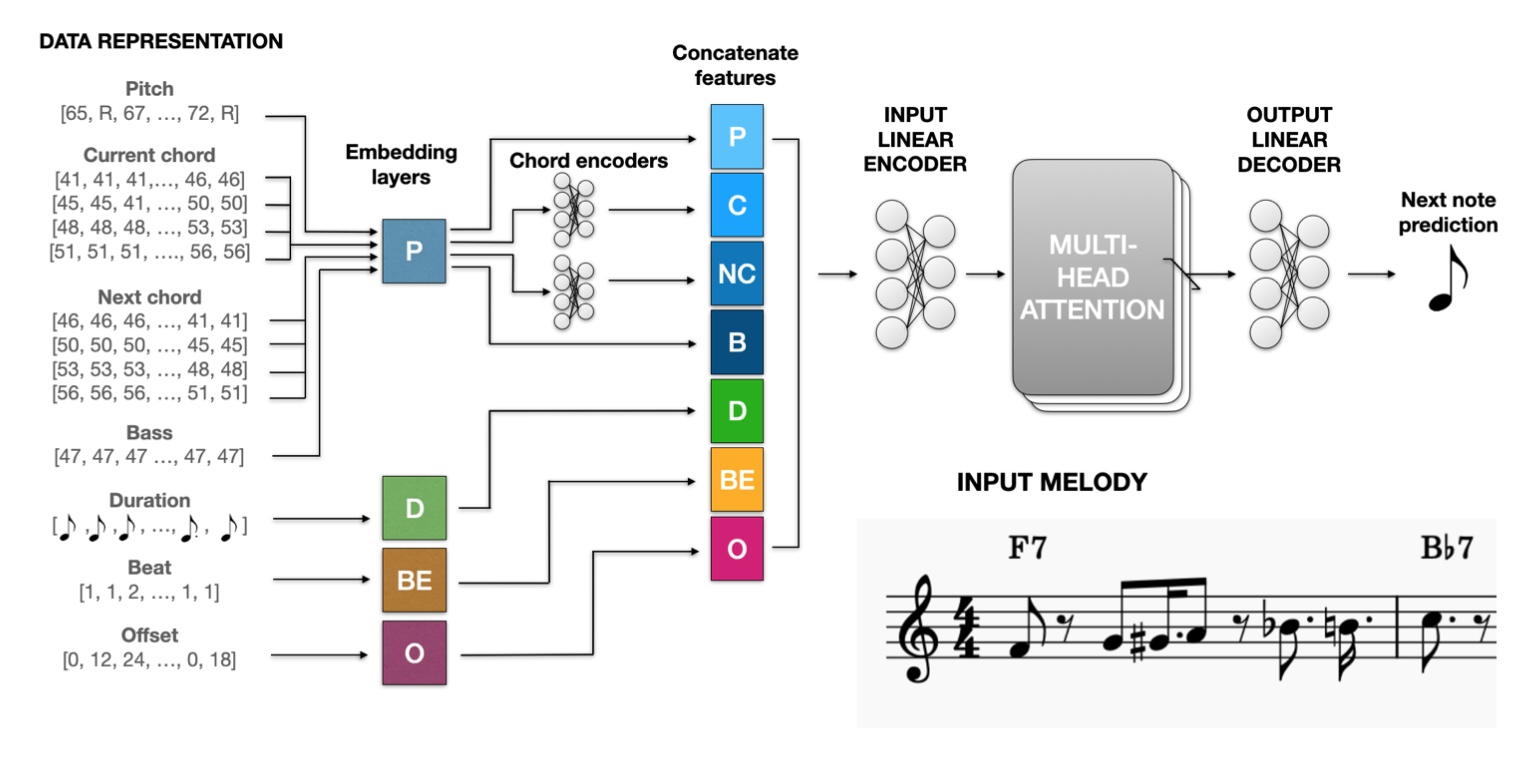
\includegraphics[width=0.5\textwidth]{Fig7.png}}
   \caption{MINGUS model architecture and data representation.}
   \label{fig:example}
\end{figure}

\noindent
MINGUS: two parallel transformer models with the same structure, predicting pitch and duration, composed by the sole encoder module with a forward mask and a pad mask.\\
The structure is the same for pitch and duration models.\\
Pitch model: D, C, B, BE, O\\
Duration model: B, BE, O\\

\section{SINTRA: LEARNING AN INSPIRATION MODEL FROM A SINGLE MULTI-TRACK MUSIC SEGMENT}
SinTra\\
(1) A novel pitch-group representation\\
(2) A novel inspiration model\\
(3) Three modules based on Transformer-XL are designed for each stage of multi-scale training to process multi-track music.\\

\noindent
Data Representation\\
Pitch-group representation
\begin{figure}[H]
	\centerline{
   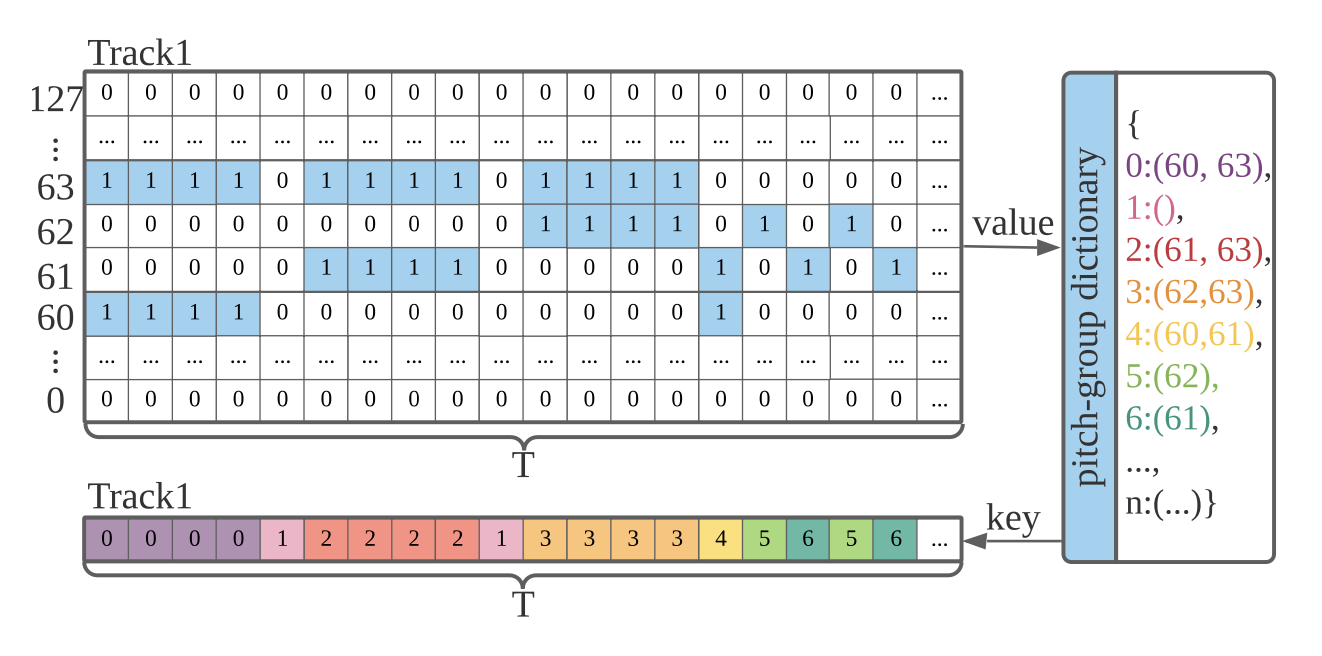
\includegraphics[width=0.5\textwidth]{Fig8.png}}
   \caption{Illustration of the pitch-group representation.}
   \label{fig:example}
\end{figure}

\noindent
Pyramid of Transformer-XL Model
\begin{figure}[H]
	\centerline{
   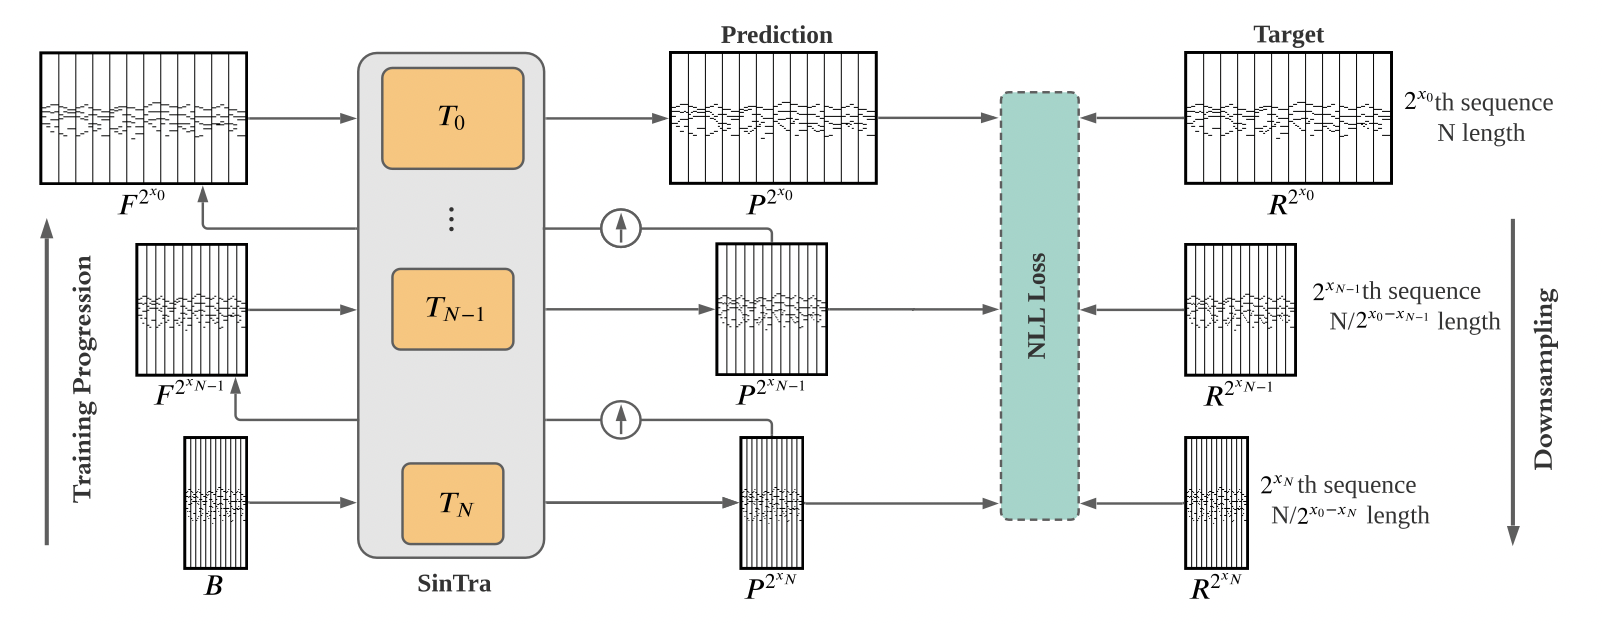
\includegraphics[width=0.5\textwidth]{Fig9.png}}
   \caption{SinTra's multi-scale pipeline.}
   \label{fig:example}
\end{figure}
\noindent
R: real music $\{R^{2^{x_0}}, ..., R^{2^{x_N}}\}$, $R^{2^{x_n}}$ is a downsampled version of $R^{2^{x_0}}$.\\
P: produced music $P^{2^n}$ is the corresponding scale of $R^{2^{x_n}}$\\
The generation of a music sample starts at the coarsest scale and sequentially passes through all models up to the finest scale.\\

\noindent
Network Structure
\begin{figure}[H]
	\centerline{
   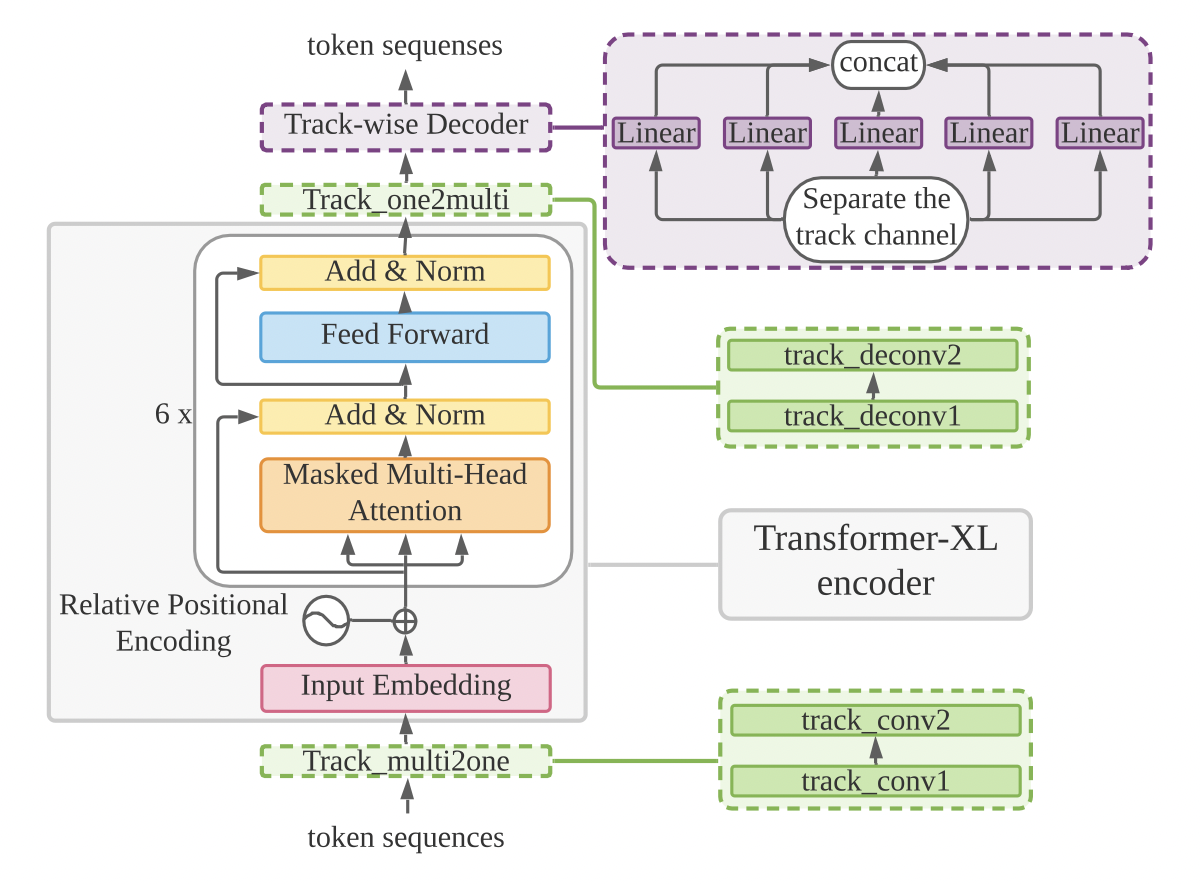
\includegraphics[width=0.5\textwidth]{Fig10.png}}
   \caption{Network structure of each scale $T_n$.}
   \label{fig:example}
\end{figure}
\noindent
Training Process
\begin{figure}[H]
	\centerline{
   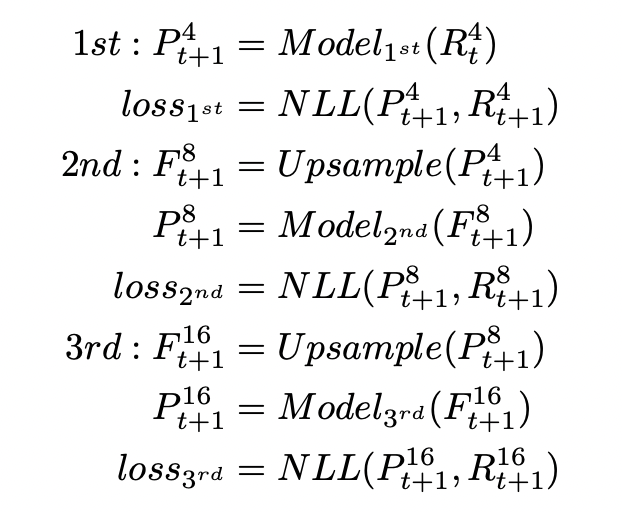
\includegraphics[width=0.4\textwidth]{Fig11.png}}
   \caption{Training process.}
   \label{fig:example}
\end{figure}

\section{COLLAGENET: FUSING ARBITRARY MELODY AND ACCOMPANIMENT INTO A COHERENT SONG}
CollageNet: given a piece of melody and an irrelevant accompanient with the same length, fuse them into harmonic two-track music. Rhythm and pitch of the melody, and chord and texture of the accompaniment.\\

\noindent
Model Architecture\\
We use the encoders of two VAEs to encode the melody and accompaniment to two latent vectors.\\
\indent
melody: $z_{mel}$, $z_{mel} = z_p \oplus {z_r}^2$ ($z_p$: pitch vector, $z_r$: rhythm vector), ${\rm EC}^2$-VAE.\\
\indent
polyphonic accompaniment: $z_{acc}$, $z_{acc} = z_c \oplus z_t$ ($z_c$: chord vector, $z_t$: texture vector).\\
Feed $z_{mel}$ and $z_{acc}$ to the actor model $G$ with transforms them into another latent vector pair $\hat{z}_{mel}$ and $\hat{z}_{acc}$. The actor model $G$ is trained under an adversarial framework together with a critic model $D$.\\
\begin{figure}[H]
	\centerline{
   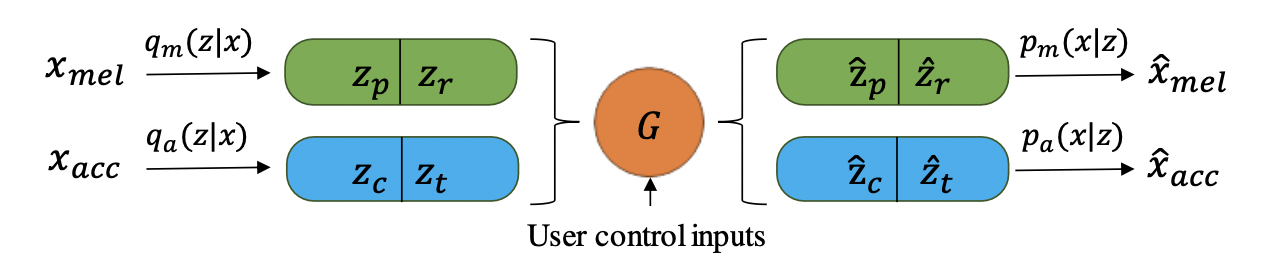
\includegraphics[width=0.7\textwidth]{Fig12.png}}
   \caption{Inference diagram.}
   \label{fig:example}
\end{figure}

\noindent
Training\\
1. pre-train the two VAEs for melodies and accompaniments.\\
2. train the $G$ and $D$ models in the latent space.\\
harmonic set ($\Omega_h$): $\{x_{mel}^{(i)},x_{acc}^{(i)}\}_{i=1}^N$\\
disharmonic set ($\Omega_{dh}$): $\{x_{mel}^{(i)},x_{acc}^{(j)}\}$ ($i \neq j$)\\
$D$ model is trained to distinguish between positivie samples and negative samples.\\
\indent
positive samples\\
\indent
$\{z_{mel}, z_{acc}\} \sim {\Omega}_h^z$\\
\indent
negative samples\\
\indent
(1) latent vectors of the disharmonic pairs $\{z_{mel},z_{acc}\} \sim \Omega_{dh}^z$\\
\indent
(2) latent vectors samples from prior $\{z_{mel},z_{acc}\} \sim p(z)$\\
\indent
(3) latent vectors produced by the actor model $G(z_{mel},z_{acc})$\\
$G$ model is trained to transform disharmonic latent vector pairs into a more harmonic pair.\\

\noindent
User Control\\
The input of the $G$ model is extended with four scalars $c_{mp}, c_{mr}, c_{ac}, c_{at} \in [0, 1]$.\\
\begin{figure}[H]
	\centerline{
   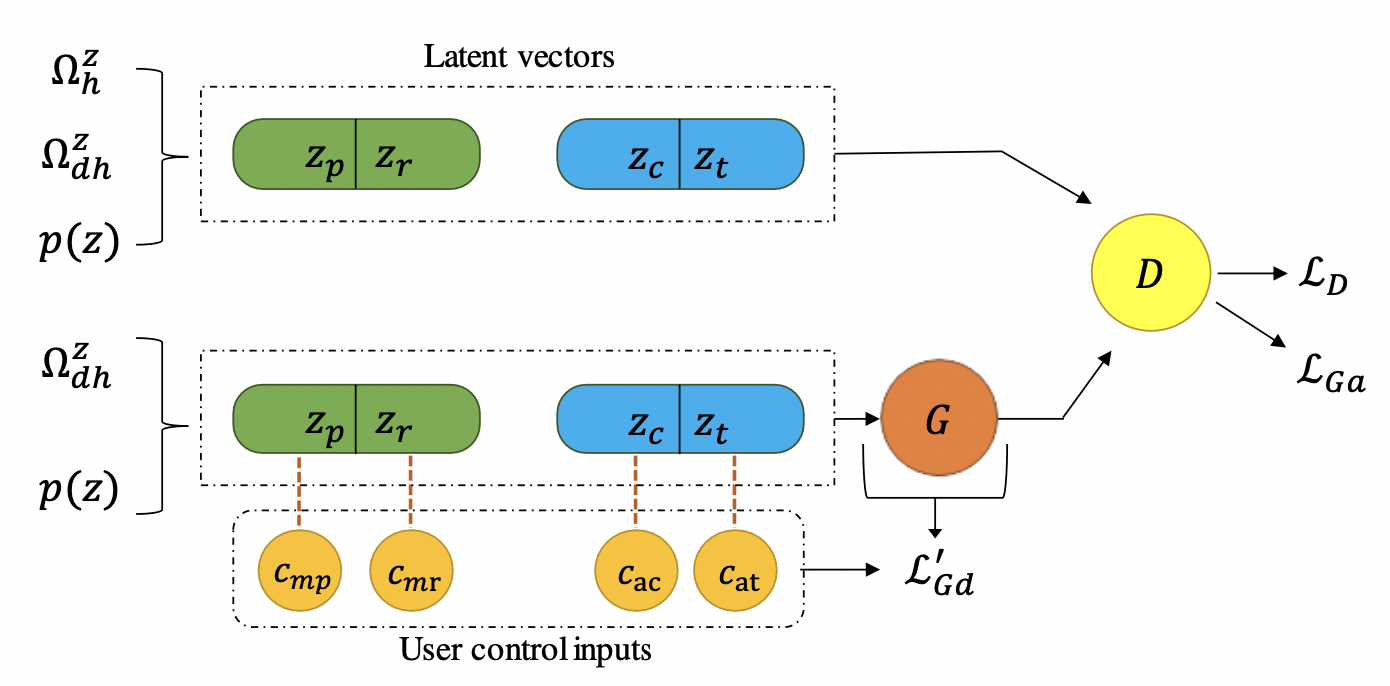
\includegraphics[width=0.7\textwidth]{Fig13.png}}
   \caption{Training diagram.}
   \label{fig:example}
\end{figure}

\section{DEEP MUSIC ANALOGY VIA LATENT REPRESENTATION DISENTANGLEMENT}
Explicitly-constrained conditional variational autoencoder (${\rm EC}^2$-VAE)\\
(1) the disentanglement is explicitly coded.\\
(2) the disentanglement does not sacrifice much of the reconstruction.\\
(3) model is capable of making analogies in the inference phrase.\\

\noindent
Analogy Algorithm\\
Any computational method capable of producing analogous versions of existing examples.\\
strict analogy algorithm: requires not only learning the representations but also disentangling them.\\
music representation learning: build a bi-directional mapping between the distributions of observation $x$ and latent representation $z$.\\

\noindent
Model Architecture
\begin{figure}[H]
	\centerline{
   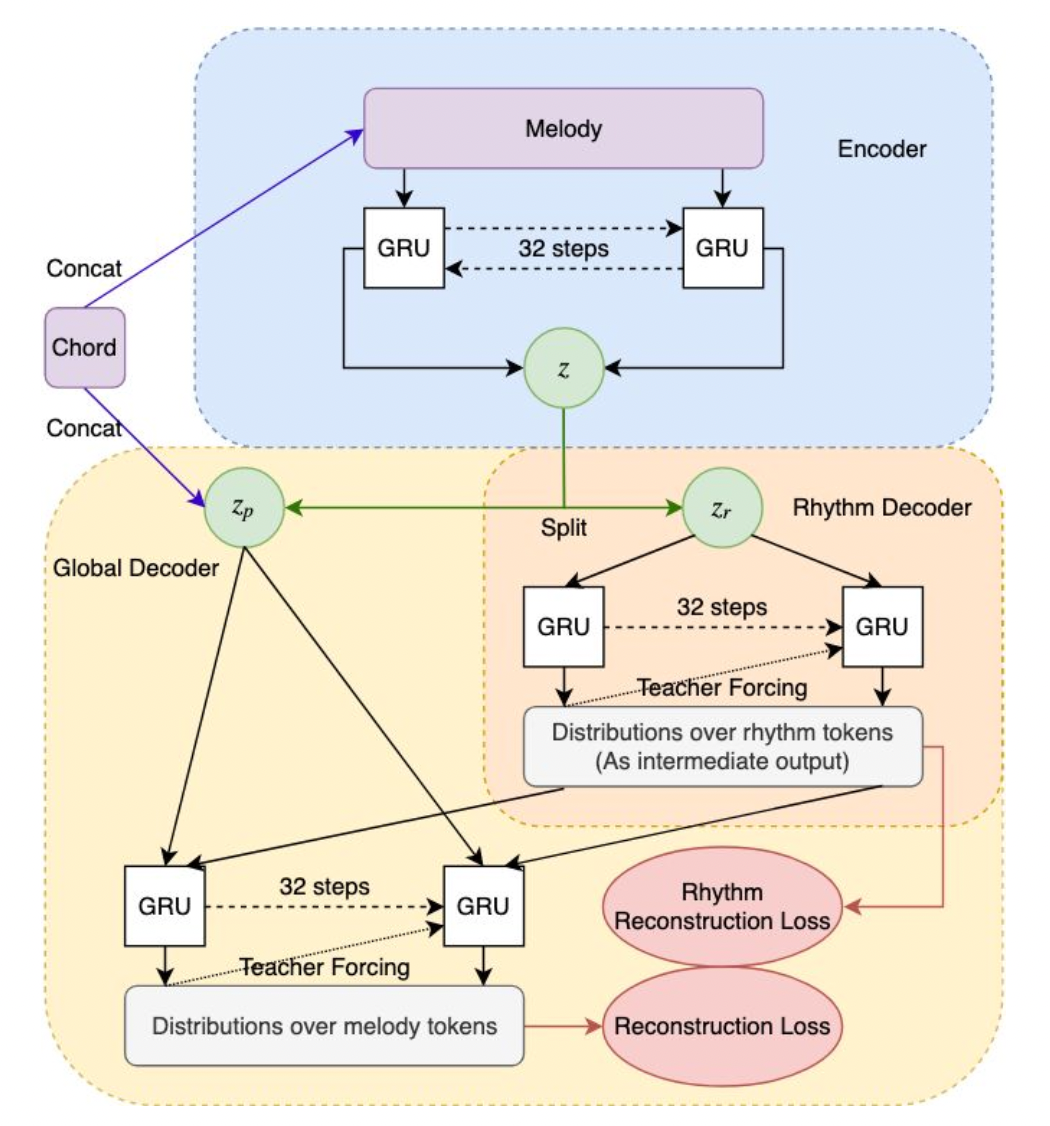
\includegraphics[width=0.4\textwidth]{Fig14.png}}
   \caption{${\rm EC}^2$-VAE model.}
   \label{fig:example}
\end{figure}

\noindent
To disentangle the latent rhythm representation $z_r$ from the overall $z$, encourage the intermediate output of $z_r$ to match the rhythm feature of the melody.\\
$z_p$ represents the other part of $z$, which is everything but rhythm.

\section{SYMBOLIC MUSIC GENERATION WITH DIFFUSION MODELS}
Denoising Diffusion Probabilistic Models (DDPMs)\\
forward process, reverse process.\\
Forward process: $q(x_t|x_{t-1}) = \mathcal{N}(x_t; \sqrt{1 - \beta_t}x_{t-1}, \beta_t I)$\\
$\Leftrightarrow$ $x_t = \sqrt{1 - \beta_t}x_{t-1} + \beta_tZ_{t-1}$ ($Z_t \sim \mathcal{N}(0, I)$)\\
$q(x_{1:N}|x_0) = \prod\limits_{t=1}^Nq(x_t|x_{t-1})$\\
Reverse process: $p_\theta(x_{t-1}; \mu_\theta(x_t,t), \sigma_\theta(x_t,t))$\\
$p_\theta(x_{0:N}) = p(x_N)\prod\limits_{t=1}^Np_\theta(x_{t-1}|x_t)$\\
Loss function\\
The training objective: $\max\limits_\theta{p_\theta(x_0)} = \int p_\theta(x_0,...,x_N)dx_{1:N}$\\
$L(\theta) = \mathbb{E}_{x_0,\epsilon,t}[{\vert \epsilon - \epsilon_\theta(\sqrt{1-\beta_t}x_0 + \sqrt{\beta}\epsilon, t) \vert}^2]$\\

\noindent
Model
\begin{figure}[H]
	\centerline{
   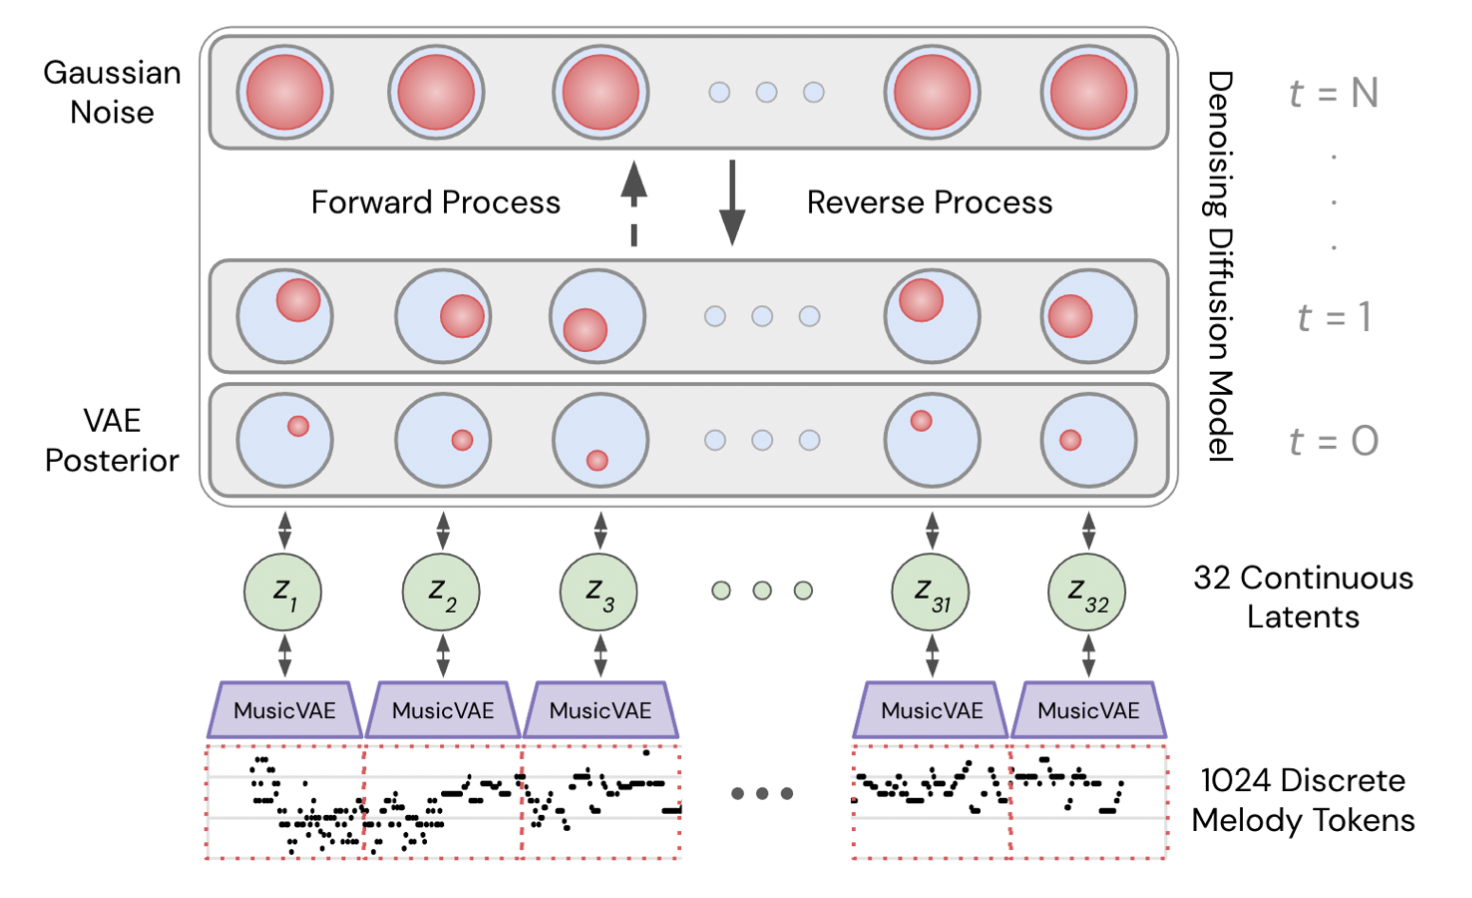
\includegraphics[width=0.5\textwidth]{Fig15.png}}
   \caption{A diagram of the diffusion model.}
   \label{fig:example}
\end{figure}
\noindent
MusicVAE embeddings\\
Transformer diffusion model: the network for $\epsilon_\theta(x_t, \sqrt{1-\beta_t})$ is a transformer.\\

\noindent
Sampling
\begin{algorithm}
	\renewcommand{\algorithmicrequire}{\textbf{Input:}}
	\renewcommand{\algorithmicensure}{\textbf{Output:}}
	\caption{Sampling}
	\label{alg:1}
	\begin{algorithmic}[H]
      \STATE $x_T \sim \mathbb{N}(0, I)$
		\FOR{$t = N, ..., 1$}
      \STATE $\epsilon \sim \mathbb{N}(0, I)$ if $t > 1$, else $\epsilon = 0$
      \STATE $x_{t-1} = \frac{1}{\sqrt{1-\beta_t}}(x_t - \frac{\beta}{\sqrt{\beta}}\epsilon_\theta(x_t,t)) + \sigma_tz$
      \ENDFOR 
      \RETURN $x_0$
	\end{algorithmic}
\end{algorithm}

\newpage
\noindent
Infilling\\
$s$ represents the partially occluded sample.
\begin{algorithm}
	\renewcommand{\algorithmicrequire}{\textbf{Input:}}
	\renewcommand{\algorithmicensure}{\textbf{Output:}}
	\caption{Infilling}
	\label{alg:2}
	\begin{algorithmic}[H]
      \REQUIRE mask $m$, sample $s$, $N$ steps, $\beta_1, ..., \beta_N$
      \STATE $x_N \sim \mathbb{N}(0, I)$
		\FOR{$t = N, ..., 1$}
      \STATE $\epsilon_1,\epsilon_2 \sim \mathbb{N}(0, I)$ if $t > 1$, else $\epsilon_1 = \epsilon_2 = 0$
      \STATE $y = \sqrt{1-\beta_t} + \sqrt{\beta_t}\epsilon_1$, if $t > 1$, else $s$
      \STATE $x_{t-1} = \frac{1}{\sqrt{1-\beta_t}}(x_t - \frac{\beta}{\sqrt{\beta}}\epsilon_z\theta(x_t,t)) + \sigma_t\epsilon_2$
      \STATE $x_{t-1} = x_{t-1} \odot (1-m) + y \odot m$
      \ENDFOR
      \RETURN $x_0$
	\end{algorithmic}
\end{algorithm}

\end{document}